\documentclass[tikz]{standalone}
\usetikzlibrary{arrows.meta}
\usetikzlibrary{bayesnet}

\begin{document}
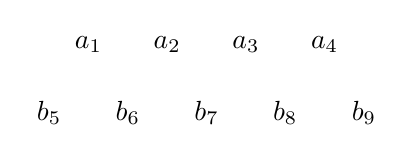
\begin{tikzpicture}
	% targets
\path
	(0,0) node (a1) {$a_1$}
	(1,0) node (a2) {$a_2$}
	(2,0) node (a3) {$a_3$}
	(3,0) node (a4) {$a_4$}
	;

\path [shift=(-120:1cm)]
	(0,0) node (b5) {$b_5$}
	(1,0) node (b6) {$b_6$}
	(2,0) node (b7) {$b_7$}
	(3,0) node (b8) {$b_8$}
	(4,0) node (b9) {$b_9$}
	;
\end{tikzpicture}
\end{document}

